\documentclass[a4paper,10pt]{report}
\usepackage[utf8]{inputenc}
\usepackage{graphicx}

% Title Page
\title{FAA partie 1}
\author{Matthieu Caron}


\begin{document}
\maketitle

\section{TP 1 : Calcul de performance}

Voici les différents résultats obtenus avec les différentes mesures de performance.
$$J_{abs} = 0.73987984094 $$
$$J_{l1} = 0.0896787983772$$
$$J_{l2} = 0.804228687838$$
$$J_{l\infty} = 2.51624302238$$



\begin{figure}[!h]
 \centering
 \caption{Comparaison entre $2*x + 3$ et les points générés}
 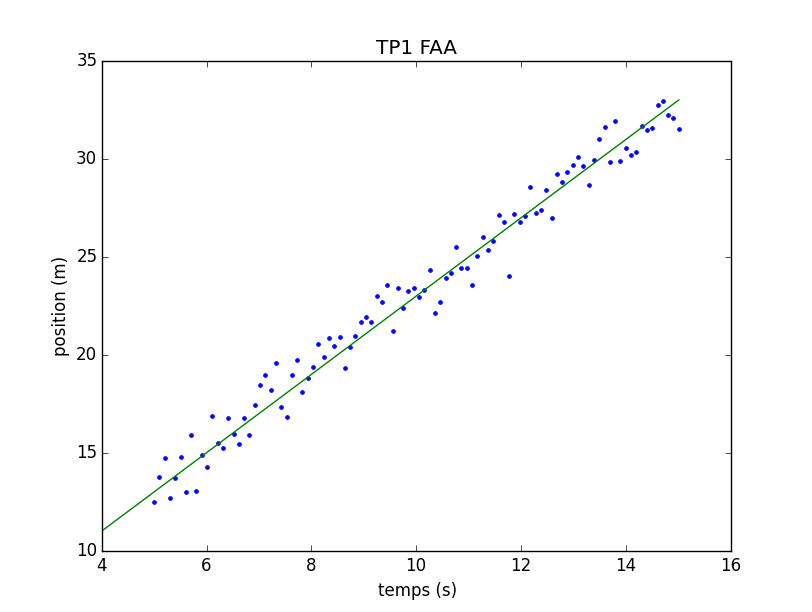
\includegraphics[width=10cm]{tp1.png}
\end{figure}

\section{TP 2 :  Moindres Carrés}
Les valeurs qui ont permis de générer les points sont 2 et 3 mais il existe un meilleur vecteur teta pour aproximer 
les points obtenus. Comme la fonction est une fonction linéaire on peut l'approximer avec les moindres carrés.
Notre fonction $2*x+3$ devient maintenant : $$1.95293789 * x + 3.59623499 $$

\begin{figure}[!h]
 \centering
 \caption{Nouvelle approximation}
 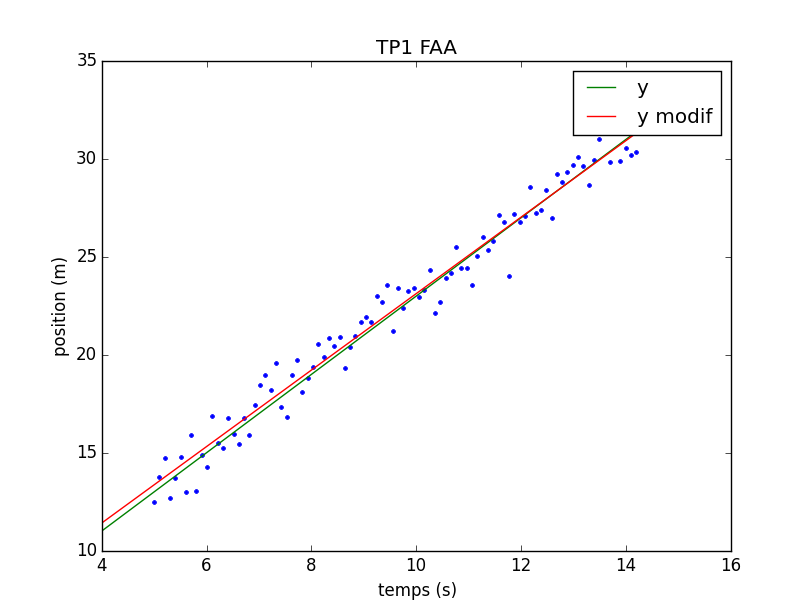
\includegraphics[width=10cm]{tp2.png}
\end{figure}

Voici les résultats des mesures de performance après les moindres carrés.
$$J_{abs} = 0.727356264922$$
$$J_{l1} = 0.0877279862436 $$
$$J_{l2} = 0.769619957035$$
$$J_{l\infty} = 2.55866627298$$

Et enfin les différences avec les résultats du tp1.

$$diff(J_{abs}) =  0.0125235760181$$
$$diff(J_{l1}) = 0.00195081213361$$
$$diff(J_{l2}) =  0.0346087308024$$
$$diff(J_{l\infty}) = 0.0424232506015$$

\section{TP 3 : Descente de gradient }
Avec la descente de gradient, on obtient 

\begin{abstract}
\end{abstract}

\end{document}          
